\section{Evolutionary Algorithms}

\begin{frame}{Evolutionary Algorithms}
\begin{figure}
  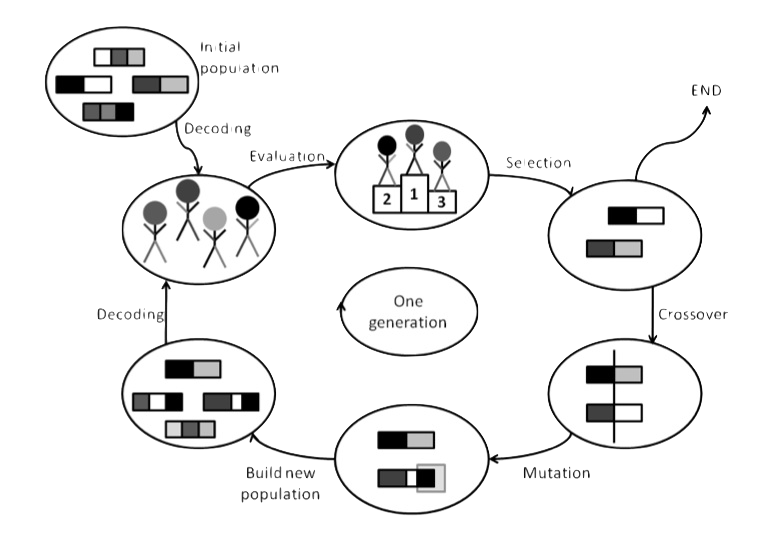
\includegraphics[width=0.8\textwidth]{img/working_principle_of_EA.png}
  \captionsetup{singlelinecheck=off,justification=raggedright}
  \caption{Schematic illustration of the evolutionary algorithm \cite[Figure 1]{Prothmann2009EvolutionaryOptimisation}}
\end{figure}
    
\end{frame}

\begin{frame}{Evolutionary Algorithms}
\begin{figure}
  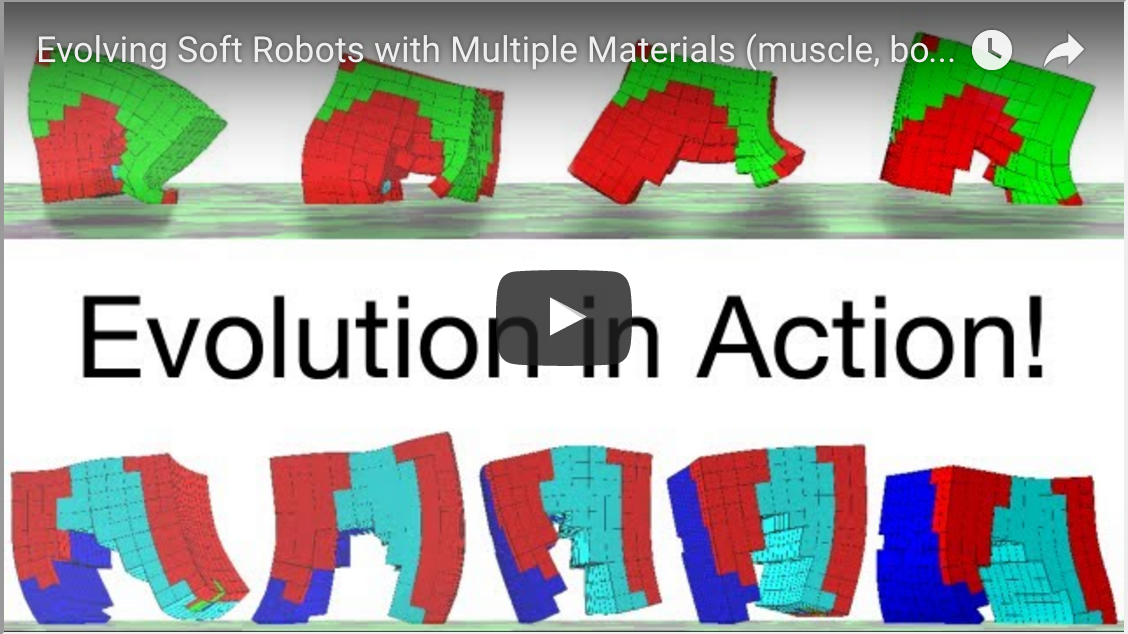
\includegraphics[width=0.8\textwidth]{img/evolution_in_action.png}
  \captionsetup{singlelinecheck=off,justification=raggedright}
\href{https://youtu.be/z9ptOeByLA4?t=1m08s}{\caption{Evolution in Action \cite{Cheney2013UnshacklingEncoding}}}
\end{figure}
\end{frame}

\begin{frame}{Evolutionary Algorithms: Glossary}
\begin{itemize}
  \item individual
  \item population
  \item fitness function
  \item selection
  \item recombination
  \item genotype
  \item phenotype
\end{itemize}
\end{frame}

\begin{frame}{Evolutionary Algorithms: Problem Statement}
  What makes an evolutionary algorithm work?
\end{frame}